\chapter{Project Management}
\label{chap:project-management}

Project management is often left as a side topic in university projects. This practice, sadly, often results in either the project not achieving its true potentials, or in worst cases catastrophic failure. It may be because of poor time management, unforseen risks for an unprepared team, a dominating project manager or the simple lack of teamwork between the team members. We believe that a GDP should have at least the following as their project management goals \cite{iansommerville2011} -

\begin{itemize}

  \item Timely delivery to the customer
  \item Meeting the customer's expectations
  \item Maintain a well-functioning development team

\end{itemize}

Shakib was the project manager for GDP 8. We are proud of the professionalism that we have demonstrated during the project. We were pragmatic in our time management, professional and honest in our communication with our supervisor and our client and finally managed our risks well. In this chapter we will analyse how we were able to achieve the above goals.

\section{Risk Analysis}
\label{sec:risk-analysis}

We will begin with risk analysis, since our management techniques evolved through our efforts of migitating the major risks. In \textbf{Table \ref{tab:risk}} we list the \textit{major} risks - those that clearly affect the project and the products we produced.

\pagebreak

\begin{center}

\begin{longtable}{ |p{5.7cm}|p{2cm}|p{2.3cm}|p{2.7cm}| }

 \hline
 	%Example of column merging
 	\multicolumn{4}{|c|}{Risk Analysis} \\
 \hline
 	%Examples of centering text
 	Risk & Affects & Probability & Effect  \\
  \hline
 	 Goals are not clear & Project, Product & Very High & Catastrophic \\
   \hline
   Software not to specification & Product & Very High & Catastrophic \\
   \hline
   Changing requirements & Project, Product & High & Serious \\
  \hline
  Team member unavailable/left & Project & Very High & Serious \\
  \hline
  Technologies unavilable, e.g. VM & Product & Very High & Serious \\
  \hline
  Underperforming software & Product & Low & Tolerable \\
  \hline
  Payment system faulty & Product & Very Low & Catastrophic \\
  \hline
  Continuous integration faulty & Product & Very Low & Tolerable \\
  \hline

\end{longtable}

%Use of captionof allows 'Table' instead of default 'Figure'
\captionof{table}{Risk Analysis}
\label{tab:risk}

\end{center}

In the following sections we discuss how we managed the risks and in turn managed our project.

\section{Time Management}
\label{sec:time-management}
Since a 4th year MEng student should spend 2/3 of their time in GDP, we estimated that, we should each spend at least 30 hours/week (out of 50 hours/week). In our previous experience we found it very difficult to keep to strict hours, because of other commitments, e.g. societies, courseworks etc.\\

To mitigate this risk, we booked a library room \textit{every weekday} for the entire 1st semester. This ensured that we always have a place to work together. We insisted on maximising our contact time, and in fact utilised the room bookings to the fullest extent by working above \textit{\textbf{30 hours}} together each week (\textbf{Appendix \ref{appendix:team-member-contribution}}).\\

We also estimated the work amount for other coursework in advance, and worked more on GDP in certain weeks. We kept our supervisor and our client well aware of our commitments each week so that we could prepare thusly. Our Gantt Chart in \textbf{Appendix \ref{appendix:gantt-charts}} demonstrates how well we followed our original plan, since work hours closely followed our initial estimates. In fact, the only change is that we finished our initial goals earlier than anticipated and could focus on further achievements like Continuous Integration(CI).

\section{Weekly Meetings}
\label{sec:weekly-meetings}
We met both the supervisor and the client at least once each week since start of the term. The goal of these meetings was to -

\begin{itemize}

  \item Demonstrate the current progress
  \item Prioritise the tasks for the following week
  \item Ensure that the client is satisfied with the direction and progress

\end{itemize}

The meetings mitigated the risk of not achieving the specification and guarded us from veering off to undesirable directions.\\

A key focus during these meetings was to clarify the project goals, deliverables and the success criteria. This made us confident in our progress each week, since we could justify our project direction during demonstrations based on the agreed success criteria from the previous meetings. We tried to be as empirical as possible in estimating our work during the meetings so that we neither over-estimated, nor under-estimated the difficulty. Not only did this helped us achieve our initial goals, but also helped us extend the deliverables to implement Synote's first attempt at continuous integration. \\

We met our client at least once more each week, in addition to continuous contact over \textit{Slack} to ensure that we were following his coding conventions, which greatly helped when we merged our code each week.

\section{Team Management}
\label{sec:people-management}
Our project manager, Shakib, focused on the following to guide his team management \cite{iansommerville2011}-

\begin{itemize}

  \item Team members gain new skills
  \item Each member feels included in the project
  \item Each member is treated idendically
  \item Manager is honest about the team's progress and the individual's contribution

\end{itemize}

The following sections better explain how the team managed the skills and tasks among themselves.

\subsection{Dividing Work}
\label{subsec:dividing-work}
The team started a weekly team meeting after the first progress seminar, after feedback from the supervisor. During this meeting we set our personal weekly tasks. Previously, task assignment was done informally.\\

Usually, after the weekly meeting (\textbf{Section \ref{sec:weekly-meetings}}), we had 4-5 different major tasks for the week. The team members that were present during the team meetings picked the tasks they preferred. Otherwise, the manager assigned a task if any member was absent or did not have a preferrence. Finally, he picked the remaining tasks.\\

During the week, if a team member finished his own task, he started others' remaining tasks if they were unavailable or helped out with ongoing ones. Similarly, if one's task depended on another's task and it was blocking the former's progress, they would either work together, or continue the other's work while they may be unavailable to work. Every effort was made to ensure that no team member spends a development day without a task.\\

\textbf{Appendix \ref{appendix:team-member-contribution}} clearly indicates each team member's individual contribution to the project, and \textbf{Appendix \ref{appendix:code-commits}} is the evidence in terms of code commits that they  produced. For example: Shakib performed nearly 60\% of the tasks of Synote's CI set up, Vlad and Tom each did 20\% of the tasks in CI, while Deepak wrote neaerly 70\% of the E2E test cases of payment feature.\\

It must be noted though - not all contribution can be measured in terms of code line commits alone, since there were significant tasks that could not be commited as code - research for example, or when collaborated code was commited from a single user. So, we have included further diagrams to clarify when a team member contributed to the project in the following sections. \\

\subsection{Collaboration}
\label{subsec:collaboration}

Even though we each had our personal tasks that we completed every week (as explained in \textbf{Section \ref{subsec:dividing-work}}), 25 - 30\% of our tasks were in fact joint effort. Similar to any well functioning software development group, we often divided our work and came together to combine our work to achieve a requirement.\\

\textbf{Appendix \ref{appendix:team-collaboration}} clearly shows timelines of each team member's major tasks throughout the project and demonstrates where and when he collaborated with others.\\

\begin{figure}[!hbt]
  	\centering
 	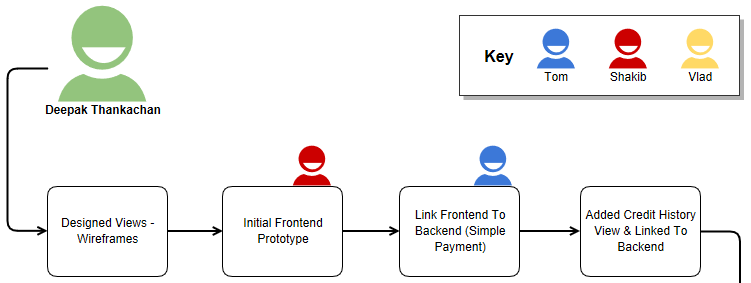
\includegraphics[width=0.8\textwidth]{deepak-collab-snip.png}
  	\caption{Example of collaboration diagram}
 	\label{fig:deepak-collaboration-snippet}
\end{figure}

For example from \textbf{Figure \ref{fig:deepak-collaboration-snippet}}, which itself is a snippet from the appendix, we know that Deepak worked with Tom to integrate the initial server side REST API for the payment feature with his front end implementation.

\subsection{Team Skills}
\label{subsec:team-skills}

A major concern was the team's lack of practical knowledge of JavaScript, specially when the entire Synote application is JavaScript based. Shakib was the most proficient in JavaScript and he worked with each team member to help them with JavaScript initially to mitigate the risk early. Similarly, the rest of the team worked hard in the first 4-5 weeks to overcome any technical difficulties, including learning promise based structures, dynamic typing, closures, and the frameworks - Sails, Angular, Protractor, Cucumber etc.\\

The team has picked up a number of development skills after this project. Tom and Vlad are more confident in their JavaScript knowledge, Deepak is fluent in front end development in Angular and HTML 5 than ever before and finally Shakib is assured of his JavaScript, Linux and team managemenet skills. Each team member also learned a significant amount about proper use of version control (See \textbf{Section \ref{sec:code-submission-process}}). The team members are also more optimistic about their individual strengths, as well as the group synergy.

\subsection{Team Inclusion and Honesty}
\label{subsec:team-inclusion}
The manager, Shakib, emphasised on equality and inclusion of team members in their contribution to the project. Each member was informed of other's contribution through a shared contribution document (\textbf{Appendix \ref{appendix:team-member-contribution}}). He also informed absent team members about group decisions after each meeting so that they feel included. Any discrepancy was openly discussed with the team member so that each team member felt equally valued, and no one wast left with unfair resentment.\\

Similarly, all team members respected other's responsibilities and even contributed to alleviate other's issues, for example: fill in the hours if someone was unavailable for a job interview.

\section{Code Quality Management}
\label{sec:code-quality-management}

We had the following goals in terms of our JavaScript coding style and quality -

\begin{itemize}

  \item Follow the industry's best practices
  \item Follow the existing practices in Synote's codebase
  \item All code must be reviewed by at least one other team member

\end{itemize}

We wanted to make sure that the client can easily add further functionality. So, we followed the conventions of Synote's lead developer. In fact, we documented the conventions we followed in the 'Contributing.md' document for Synote so that the future developers also follow the same conventions.\\

As discussed before, code produced during pair programming was continuously reviewed by both team members. Similarly Shakib reviewed all code written by the team members before submitting the code to the client each week. Static checks to find usual JavaScript issues that may indicate bugs e.g. undeclared/unused variables etc. were also marked by 'linters' provided in the IDEs used. We also achieved almost complete test coverage in the payment feature through server side unit/integration and E2E tests (\textbf{Appendix \ref{appendix:server-test-cases}} and \textbf{\ref{appendix:e2e-testing}}). Finally, the client also provided feedback about the code we submitted and we refactored accordingly, for example: use of services in the client, promises throughout the application etc.

\section{Code Submission Process}
\label{sec:code-submission-process}

We had the following goals in terms of code submissions -

\begin{itemize}

  \item Submit code to client weekly
  \item Commit often
  \item Review often
  \item Reduce merge conflicts

\end{itemize}

In order to achieve the goals, we adopted a code submission strategy (\textbf{Figure \ref{fig:version-control}}). Shakib forked both the client's E2E testing and application repositories to create GDP8 repositories. The master branch of the GDP8 repositories were regarded stable and no direct commits were made on master branches. Instead feature branches were created from the GDP8 master branches, and each developer submitted code to the feature branch every day. At the end of the day, there would be no work left to be submitted to the feature branch.\\

\begin{figure}[!hbt]
  	\centering
 	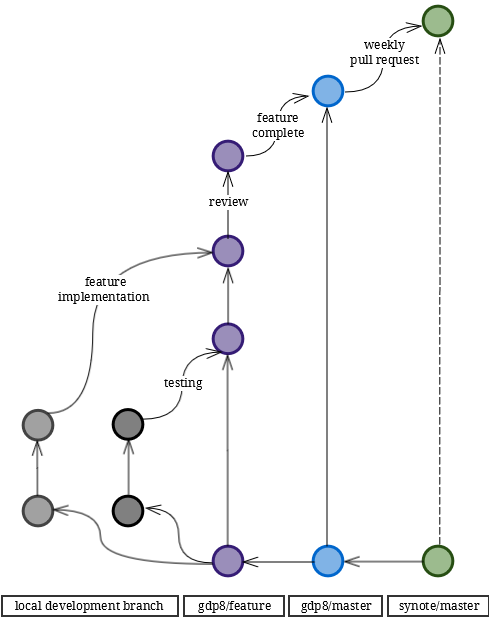
\includegraphics[width=0.8\textwidth]{commits.png}
  	\caption{Version Control}
 	\label{fig:version-control}
\end{figure}

Once a feature was nearly complete, code review was performed on the feature branches. On Fridays, Shakib pushed the stable code on GDP8 master brances, merged with the latest client's master branch and finally re-ran all the tests. This ensured that the client had minimal effort in merging our one week's worth of code. In fact, we had \textbf{\textit{no conflicts}} in submitting our code to the client and did not break any functionality on the client's existing repositories, even when there were multiple other groups working on the same repositories.
